% !TEX TS-program = pdflatex
% !TEX encoding = UTF-8 Unicode

% This is a simple template for a LaTeX document using the ``article'' class.
% See ``book'', ``report'', ``letter'' for other types of document.

\documentclass[11pt]{article} % use larger type; default would be 10pt

\usepackage[utf8]{inputenc} % set input encoding (not needed with XeLaTeX)

%%% Examples of Article customizations
% These packages are optional, depending whether you want the features they provide.
% See the LaTeX Companion or other references for full information.

%%% PAGE DIMENSIONS
\usepackage{geometry} % to change the page dimensions
\geometry{a4paper} % or letterpaper (US) or a5paper or....
\geometry{margin=1in} % for example, change the margins to 2 inches all round
% \geometry{landscape} % set up the page for landscape
%   read geometry.pdf for detailed page layout information

\usepackage{graphicx} % support the \includegraphics command and options

% \usepackage[parfill]{parskip} % Activate to begin paragraphs with an empty line rather than an indent

%%% PACKAGES
\usepackage{booktabs} % for much better looking tables
\usepackage{array} % for better arrays (eg matrices) in maths
\usepackage{paralist} % very flexible & customisable lists (eg. enumerate/itemize, etc.)
\usepackage{verbatim} % adds environment for commenting out blocks of text & for better verbatim
\usepackage{subfig} % make it possible to include more than one captioned figure/table in a single float
% These packages are all incorporated in the memoir class to one degree or another...
\usepackage{enumitem}
\usepackage{amsmath}

% para los cuadritos en links
%\usepackage[linkbordercolor={0 0 1}, citebordercolor={0 1 0}, urlbordercolor={1 0 0}]{hyperref}
\usepackage[colorlinks=true, linkcolor=black, citecolor=green, urlcolor=red]{hyperref} % solo resalta
\usepackage[spanish]{babel}



%%% HEADERS & FOOTERS
\usepackage{fancyhdr} % This should be set AFTER setting up the page geometry
\pagestyle{fancy} % options: empty , plain , fancy
\renewcommand{\headrulewidth}{0pt} % customise the layout...
\lhead{}\chead{}\rhead{}
\lfoot{}\cfoot{\thepage}\rfoot{}

%%% SECTION TITLE APPEARANCE
\usepackage{sectsty}
\allsectionsfont{\sffamily\mdseries\upshape} % (See the fntguide.pdf for font help)
% (This matches ConTeXt defaults)

%%% ToC (table of contents) APPEARANCE
\usepackage[nottoc,notlof,notlot]{tocbibind} % Put the bibliography in the ToC
\usepackage[titles,subfigure]{tocloft} % Alter the style of the Table of Contents
\renewcommand{\cftsecfont}{\rmfamily\mdseries\upshape}
\renewcommand{\cftsecpagefont}{\rmfamily\mdseries\upshape} % No bold!

%%% END Article customizations

%%% The ``real'' document content comes below...

\title{Trabajo práctico 1\\ Redes Neuronales y Aprendizaje Profundo}
\author{Ignacio Ezequiel Cavicchioli\\Padrón 109428\\icavicchioli@fi.uba.ar}
\date{10/9/2025} % Activate to display a given date or no date (if empty),
         % otherwise the current date is printed



\begin{document}
\maketitle

\tableofcontents



\section{Introducción}

Este documento presenta el desarrollo de las consignas del trabajo práctico N°2 de la materia de \textbf{Redes Neuronales y Aprendizaje Profundo}.  El código correspondiente fue realizado en  \textit{Jupyter notebooks}, \textit{Python}, adjuntados a la entrega en formato PDF. Toda imagen o implementación requeridas para el análisis se explicitarán en el presente archivo, por lo que la lectura del código en sí queda a discreción del lector. La teoría relevante será presentada y discutida en la sección pertinente.


\newpage

\section{Ejercicio 1}

\subsection{Consignas}

Implemente un perceptrón simple que aprenda la función lógica AND y la función lógica OR, de 2 y de 4 entradas. Muestre la evolución del error durante el entrenamiento. Para el caso de 2 dimensiones, grafique la recta discriminadora y todos los vectores de entrada de la red.

\subsection{Desarrollo}

Lo primero que se hizo fue generar el dataset para entrenar los perceptrones, que no es más que la tabla de verdad de la función lógica que se quiere aprender.

Las figuras \ref{fig:and2err}, \ref{fig:and4},\ref{fig:or2err} y \ref{fig:or4} muestran el error en función de la iteración (de entrenamiento) para los perceptrones que emulan las funciones AND y OR de 2 y 4 entradas. Como se discutió en la teórica, el perceptrón es capaz de aprender estas funciones lógicas simples, por lo que el error final del entrenamiento es cero.

La figura \ref{fig:orfront} muestra la frontera de decisión del perceptrón que aprendió la función OR, y la \ref{fig:frontAND} muestra la frontera para la compuerta AND. Los puntos del mismo color son de la misma clase (0 o 1), y son adecuadamente segregados por la frontera. Contrario a SVM, el perceptrón simple no tiene la distancia desde la frontera hasta las muestras en su función de costo, por lo que la recta que separa las clases no es única.

Para encontrar la fórmula de la recta que hace de frontera de decisión se puede partir de la expresión de la sumatoria de los $X$ con sus respectivos pesos y el bias, y suponer que $Y=0$, lo que significa que estás parado sobre la frontera, tu muestra no es ni de una clase ni de la otra.

$$
X1 \cdot w1 + X2 \cdot w2 + b = 0
$$

Si suponemos que $X1$ es nuestra abscisa que vamos a barrer y $X2$ es la ordenada, la recta toma la forma de:

$$
X2 = \frac{w1 \cdot X1 + b}{-w2}
$$

Y entonces $m=-w1/w2 $ y b = $-b/w2$

\begin{figure}[h!]
	\centering
	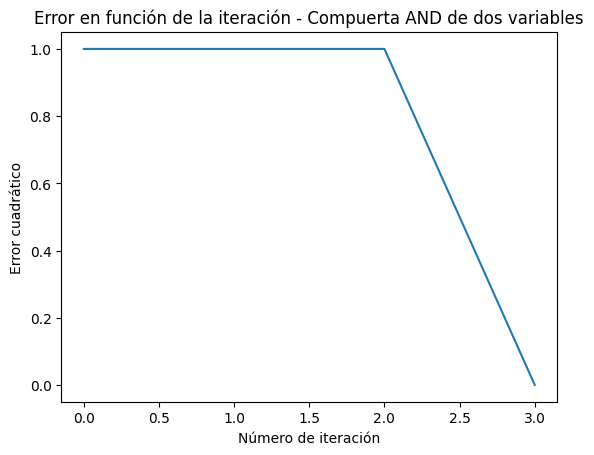
\includegraphics[width=0.7\linewidth]{../imgs/ej1/AND2err}
	\caption[]{Error de entrenamiento en el tiempo para compuerta AND de 2 entradas}
	\label{fig:and2err}
\end{figure}


\begin{figure}[h!]
	\centering
	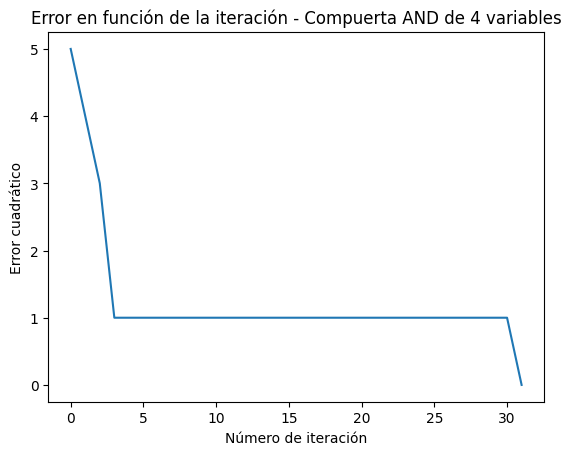
\includegraphics[width=0.7\linewidth]{../imgs/ej1/AND4}
	\caption[]{Error de entrenamiento en el tiempo para compuerta AND de 4 entradas}
	\label{fig:and4}
\end{figure}


\begin{figure}[h!]
	\centering
	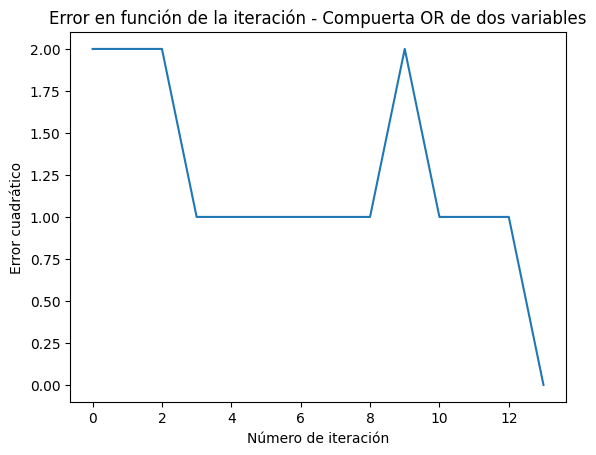
\includegraphics[width=0.7\linewidth]{../imgs/ej1/OR2err}
	\caption[]{Error de entrenamiento en el tiempo para compuerta OR de 2 entradas}
	\label{fig:or2err}
\end{figure}

\begin{figure}[h!]
	\centering
	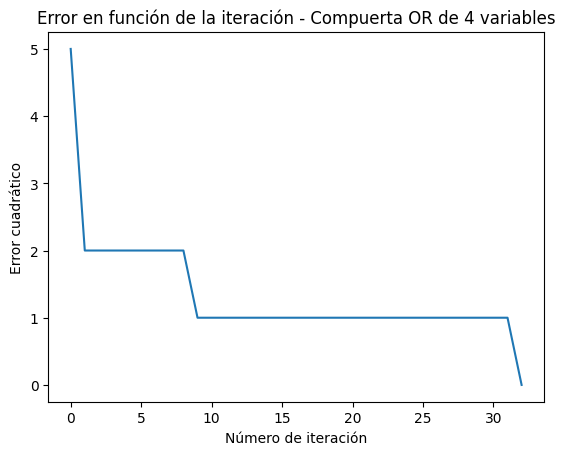
\includegraphics[width=0.7\linewidth]{../imgs/ej1/OR4}
	\caption[]{Error de entrenamiento en el tiempo para compuerta OR de 4 entradas}
	\label{fig:or4}
\end{figure}

\begin{figure}[h!]
	\centering
	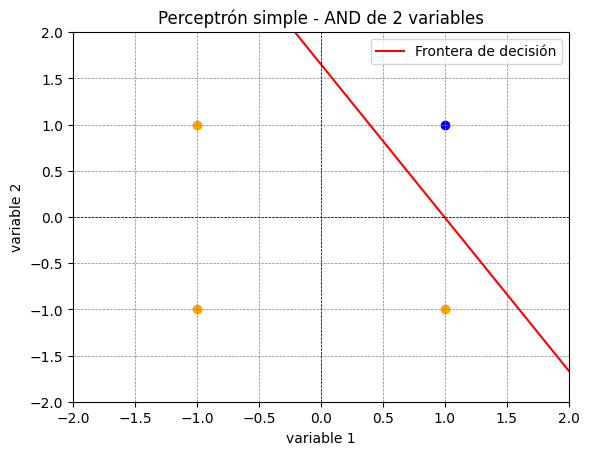
\includegraphics[width=0.7\linewidth]{../imgs/ej1/ANDFRONT}
	\caption[]{Frontera encontrada para compuerta AND de 2 entradas}
	\label{fig:frontAND}
\end{figure}



\begin{figure}[h!]
	\centering
	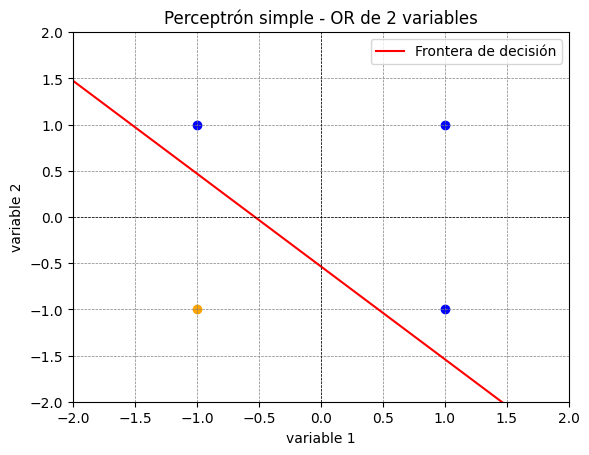
\includegraphics[width=0.7\linewidth]{../imgs/ej1/ORFRONT}
	\caption[]{Frontera encontrada para compuerta OR de 2 entradas}
	\label{fig:orfront}
\end{figure}


\subsection{Análisis}

Los perceptrones lograron aprender sus funciones lógicas designadas sin error y en una cantidad finita de iteraciones del algoritmo. Esto es el resultado esperado, se sabe que puede aprender este tipo particular de problemas.

Una parte interesante del ejercicio fue el armado del algoritmo de gradiente descendiente, regla por la cual el perceptrón va moviendo su frontera de decisión. Los gráficos muestran un error decreciente en el tiempo, que a veces aumenta espuriamente para luego ser corregido, porque el gradiente descendiente va actualizando los pesos en función del error, intentando moverse hacia fronteras que predigan correctamente.

La obtención de la recta que hace de frontera en 2D solo requirió del desarrollo de fórmulas hecho en la sección previa.

En líneas generales, el ejercicio sirvió como una buena introducción a los perceptrones y el concepto de gradiente descendiente.


\clearpage

\section{Ejercicio 2}

\subsection{Consignas}

Determine numéricamente cómo varía la capacidad del perceptrón simple en función del número de patrones enseñados.


\subsection{Desarrollo}

La capacidad de un perceptrón está definida en la p.111 (expresión 5.63) del libro ``Introduction to the theory of neural computation''. La idea es básicamente determinar la cantidad de patrones aleatorios (con etiqueta aleatoria) para el cual existe una frontera. En el libro se demuestra que la capacidad de almacenamiento máxima del perceptrón converge a $p_{max} = 2N$, con $p$ la cantidad de patrones y N, el número de pesos sinápticos que tiene el perceptrón (o cantidad de unidades de entrada), con $N \to \inf$.

Para corroborar experimentalmente esta aserción, se entrenó un perceptrón de un N particular con cada vez más patrones y se registró el resultado, para luego graficarlo.

En pocas palabras, el código genera conjuntos de patrones aleatorios y entrena un perceptrón simple para clasificarlos. Repite el experimento múltiples veces\footnote{Para un cierto $p$ se hacen varios experimentos y se promedia, por eso hay una cantidad de unidades de entrada y de repeticiones} y calcula con qué frecuencia el perceptrón logra aprender sin errores (es decir, converge). Luego grafica la probabilidad de éxito en función de $\alpha = \frac{p}{N}$, donde $p$ es la cantidad de patrones y $N$ la dimensión de entrada, mostrando así la capacidad del perceptrón. Se espera que la recta vertical $p/N = 2$ interseque la gráfica en $p=1/2$ (como en la literatura citada).


los resultados para $N=30$ se pueden ver en la figura \ref{fig:capacidad}, y para $N=10$, en la \ref{fig:N10}. No se hizo con más unidades de entrada porque condiciona mucho el tiempo de ejecución y la cantidad de epochs necesarias para lograr un buen resultado.

\begin{figure}[htbp!]
	\centering
	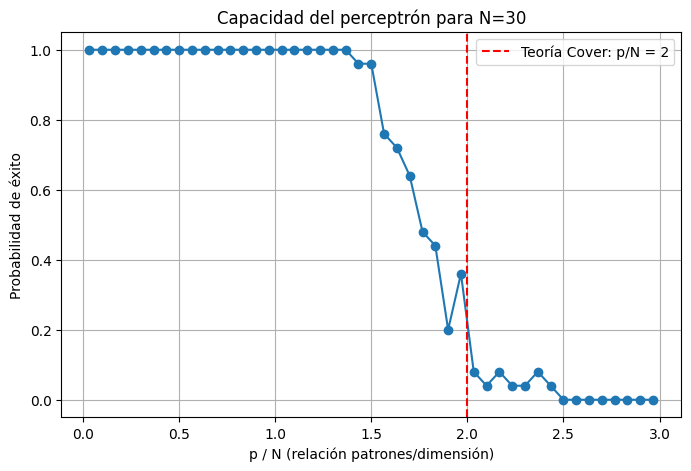
\includegraphics[width=0.7\linewidth]{../imgs/ej2/capacidad}
	\caption[]{Ensayo de capacidad $N=30$}
	\label{fig:capacidad}
\end{figure}

\begin{figure}[htbp!]
	\centering
	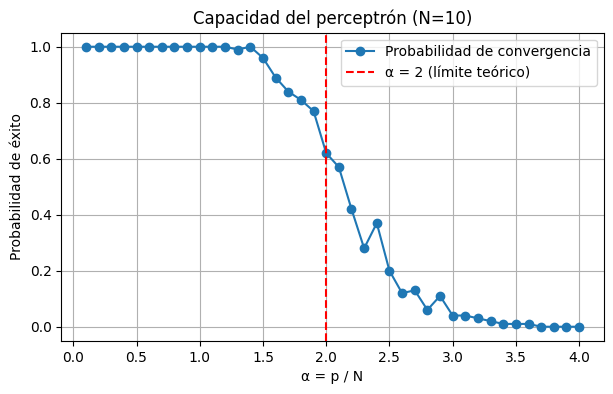
\includegraphics[width=0.7\linewidth]{../imgs/ej2/N10}
	\caption[]{Ensayo de capacidad $N=10$}
	\label{fig:N10}
\end{figure}

\newpage

\subsection{Análisis}

La figura \ref{fig:capacidad} muestra que la capacidad de memorizar (el eje Y) del perceptrón es perfecta (vale 1) y, a medida que aumenta la cantidad de patrones, decrece hasta hacerse cero. El cruce por el punto $p/N =2$ se da aproximadamente en $p\simeq 0.5$, resultado coincidente con la teoría del libro mencionado.

La transición, o flanco, no es perfectamente vertical, sino que decrece casi como una función sigmoidea. Esto es debido al uso de valores de $N$ relativamente pequeños. A forma comparativa se incluye la imagen \ref{fig:N10}, de $N=10$. En esta se ve que la capacidad tarda más en converge a cero (en $N=30$ se hace cero en $2.5$, y en $N=10$, en $3.5$), y la intersección del límite teórico es más cercana a $0.6$ y no $0.5$.

Resumiendo, aún con las limitaciones en la cantidad de unidades de entrada, se empieza a divisar una tendencia que parece coincidir con la teoría.



\clearpage

\section{Ejercicio 3}

\subsection{Consignas}

Implemente un perceptrón multicapa que aprenda la función lógica XOR de 2 y de 4 entradas (utilizando el algoritmo Backpropagation y actualizando en batch). Muestre cómo evoluciona el error durante el entrenamiento.

\subsection{Desarrollo}

En este inciso se entrenó un MLP para que aprendan la XOR, pero se hizo con 2, 4 y 10 neuronas en la capa oculta. La idea general fue crear las tablas de verdad de las funciones XOR de 2 y 4 entradas y entrenar MLP´s, registrando el error en función de las epochs.

\subsubsection{2 Neuronas en capa oculta}

En este primer caso se utilizó un perceptrón multicapa con una capa oculta de dos neuronas, con el objetivo de que aprenda la función XOR.
Se trabajó tanto con la XOR de dos entradas como con la de cuatro entradas, manteniendo la misma arquitectura a fin de observar las diferencias en la capacidad de representación del modelo.

Para la XOR de dos entradas, la red logró converger correctamente, alcanzando un error cercano a cero y reproduciendo exactamente la tabla de verdad de la función.
En las Figuras~\ref{fig:xor2err} y~\ref{fig:xor2front} se muestra la evolución del error por época y la frontera de decisión obtenida, respectivamente, donde puede verse una separación clara entre las clases.

En contraste, al aplicar la misma arquitectura a la XOR de cuatro entradas, la red no consiguió reducir el error a valores cercanos a cero, incluso habiendo hasta triplicado la cantidad de epochs. (Figura~\ref{fig:xor4err}).

Esto apunta a que dos neuronas ocultas no son suficientes para modelar la complejidad de la XOR de cuatro entradas, y se supone que se debe principalmente al incremento exponencial en cantidad de combinaciones posibles. La red ya no dispone de capacidad suficiente como para memorizar los patrones, siendo esto una manifestación práctica de la capacidad teórica analizada en el ejercicio anterior.


\begin{figure}[htbp!]
	\centering
	\includegraphics[width=0.7\linewidth]{"../imgs/ej3/2 neur int/xor2_err"}
	\caption{Error por época - XOR de 2 entradas - MLP 2 neuronas en capa oculta}
	\label{fig:xor2err}
\end{figure}

\begin{figure}[htbp!]
	\centering
	\includegraphics[width=0.7\linewidth]{"../imgs/ej3/2 neur int/xor2_front"}
	\caption{Frontera de decisión - XOR de 2 entradas - MLP 2 neuronas en capa oculta}
	\label{fig:xor2front}
\end{figure}

\begin{figure}[htbp!]
	\centering
	\includegraphics[width=0.7\linewidth]{"../imgs/ej3/2 neur int/xor4_err"}
	\caption{Error por época - XOR de 4 entradas - MLP 2 neuronas en capa oculta}
	\label{fig:xor4err}
\end{figure}

\begin{table}[h!]
	\centering
	\begin{tabular}{cccc}
		\hline
		\textbf{Entradas} & \textbf{Target} & \textbf{Salida sigmoide} & \textbf{Predicción (umbral 0.5)} \\
		\hline
		$[0\ 0]$ & 0 & 0.082 & 0 \\
		$[0\ 1]$ & 1 & 0.927 & 1 \\
		$[1\ 0]$ & 1 & 0.927 & 1 \\
		$[1\ 1]$ & 0 & 0.077 & 0 \\
		\hline
	\end{tabular}
	\caption{Resultados del perceptrón con dos entradas  - MLP 2 neuronas en capa oculta}
\end{table}

\begin{table}[h!]
	\centering
	\begin{tabular}{cccc}
		\hline
		\textbf{Entradas} & \textbf{Target} & \textbf{Salida sigmoide} & \textbf{Predicción (umbral 0.5)} \\
		\hline
		$[-1\ -1\ -1\ -1]$ & 0 & 0.725 & 1 \\
		$[1\ -1\ -1\ -1]$ & 1 & 0.837 & 1 \\
		$[-1\ 1\ -1\ -1]$ & 1 & 0.701 & 1 \\
		$[1\ 1\ -1\ -1]$ & 0 & 0.036 & 0 \\
		$[-1\ -1\ 1\ -1]$ & 1 & 0.708 & 1 \\
		$[1\ -1\ 1\ -1]$ & 0 & 0.048 & 0 \\
		$[-1\ 1\ 1\ -1]$ & 0 & 0.045 & 0 \\
		$[1\ 1\ 1\ -1]$ & 0 & 0.009 & 0 \\
		$[-1\ -1\ -1\ 1]$ & 1 & 0.879 & 1 \\
		$[1\ -1\ -1\ 1]$ & 0 & 0.063 & 0 \\
		$[-1\ 1\ -1\ 1]$ & 0 & 0.030 & 0 \\
		$[1\ 1\ -1\ 1]$ & 0 & 0.029 & 0 \\
		$[-1\ -1\ 1\ 1]$ & 0 & 0.055 & 0 \\
		$[1\ -1\ 1\ 1]$ & 0 & 0.036 & 0 \\
		$[-1\ 1\ 1\ 1]$ & 0 & 0.011 & 0 \\
		$[1\ 1\ 1\ 1]$ & 0 & 0.027 & 0 \\
		\hline
	\end{tabular}
	\caption{Resultados del perceptrón con cuatro entradas  - MLP 2 neuronas en capa oculta}
\end{table}

\clearpage

\subsubsection{4 Neuronas en capa oculta}

En este caso se incrementó el número de neuronas en la capa oculta a cuatro, con el objetivo de mejorar la capacidad de representación del MLP.
Para la XOR de dos entradas, la red continúa convergiendo correctamente, alcanzando un error muy bajo y generando fronteras de decisión suaves y bien definidas (Figuras~\ref{fig:ecm2} y~\ref{fig:front2}).
Esto se refleja también en la tabla de resultados, donde todas las predicciones coinciden con los valores esperados.

Para la XOR de cuatro entradas, aunque el error global se reduce ligeramente en comparación con la red de dos neuronas, la red aún no logra converger a un error nulo (Figura~\ref{fig:ecm4}).
La complejidad de la función sigue superando la capacidad de la red, aunque se observa que las fronteras de decisión empiezan a tomar formas curvas que intentan separar mejor las clases.
Esto evidencia que un aumento en el número de neuronas mejora la capacidad de representación, pero todavía no es suficiente para clasificar correctamente todas las combinaciones de la XOR de cuatro entradas.
En la tabla correspondiente se puede ver que varias predicciones todavía difieren del target esperado.


\begin{figure}[htbp!]
	\centering
	\includegraphics[width=0.7\linewidth]{"../imgs/ej3/4 neur int/ecm2"}
	\caption{Error por época - XOR de 2 entradas - MLP 4 neuronas en capa oculta}
	\label{fig:ecm2}
\end{figure}

\begin{figure}[htbp!]
	\centering
	\includegraphics[width=0.7\linewidth]{"../imgs/ej3/4 neur int/front2"}
	\caption{Frontera de decisión - XOR de 2 entradas - MLP 4 neuronas en capa oculta}
	\label{fig:front2}
\end{figure}

\begin{figure}[htbp!]
	\centering
	\includegraphics[width=0.7\linewidth]{"../imgs/ej3/4 neur int/ecm4"}
	\caption{Error por época - XOR de 4 entradas - MLP 4 neuronas en capa oculta}
	\label{fig:ecm4}
\end{figure}





\begin{table}[h!]
	\centering
	\begin{tabular}{cccc}
		\hline
		\textbf{Entradas} & \textbf{Target} & \textbf{Salida sigmoide} & \textbf{Predicción (umbral 0.5)} \\
		\hline
		$[0\ 0]$ & 0 & 0.059 & 0 \\
		$[0\ 1]$ & 1 & 0.902 & 1 \\
		$[1\ 0]$ & 1 & 0.946 & 1 \\
		$[1\ 1]$ & 0 & 0.102 & 0 \\
		\hline
	\end{tabular}
	\caption{Resultados del perceptrón con dos entradas - MLP 4 neuronas en capa oculta}
\end{table}


\begin{table}[h!]
	\centering
	\begin{tabular}{cccc}
		\hline
		\textbf{Entradas} & \textbf{Target} & \textbf{Salida sigmoide} & \textbf{Predicción (umbral 0.5)} \\
		\hline
		$[-1\ -1\ -1\ -1]$ & 0 & 0.727 & 1 \\
		$[1\ -1\ -1\ -1]$ & 1 & 0.879 & 1 \\
		$[-1\ 1\ -1\ -1]$ & 1 & 0.697 & 1 \\
		$[1\ 1\ -1\ -1]$ & 0 & 0.033 & 0 \\
		$[-1\ -1\ 1\ -1]$ & 1 & 0.863 & 1 \\
		$[1\ -1\ 1\ -1]$ & 0 & 0.054 & 0 \\
		$[-1\ 1\ 1\ -1]$ & 0 & 0.039 & 0 \\
		$[1\ 1\ 1\ -1]$ & 0 & 0.010 & 0 \\
		$[-1\ -1\ -1\ 1]$ & 1 & 0.696 & 1 \\
		$[1\ -1\ -1\ 1]$ & 0 & 0.028 & 0 \\
		$[-1\ 1\ -1\ 1]$ & 0 & 0.058 & 0 \\
		$[1\ 1\ -1\ 1]$ & 0 & 0.003 & 0 \\
		$[-1\ -1\ 1\ 1]$ & 0 & 0.034 & 0 \\
		$[1\ -1\ 1\ 1]$ & 0 & 0.007 & 0 \\
		$[-1\ 1\ 1\ 1]$ & 0 & 0.003 & 0 \\
		$[1\ 1\ 1\ 1]$ & 0 & 0.003 & 0 \\
		\hline
	\end{tabular}
	\caption{Resultados del perceptrón con cuatro entradas - MLP 4 neuronas en capa oculta}
\end{table}

\clearpage

\subsubsection{10 Neuronas en capa oculta}

Al aumentar el número de neuronas en la capa oculta a diez, se observa un cambio significativo en el comportamiento del MLP.
Para la XOR de dos entradas, la red sigue convergiendo sin problemas y mantiene fronteras de decisión suaves y bien definidas (Figura~\ref{fig:2ecm}).

Para la XOR de cuatro entradas, a diferencia de los casos anteriores con 2 o 4 neuronas, ahora la red logra aprender correctamente todos los patrones, alcanzando un error muy bajo (Figura~\ref{fig:4ecm}).
Las fronteras de decisión siguen siendo curvas (Figura~\ref{fig:front}), lo que indica que la función sigue siendo no lineal, pero la mayor cantidad de neuronas le proporciona la capacidad suficiente para representar correctamente la XOR de cuatro entradas.
Esto confirma que las dificultades observadas en los experimentos anteriores estaban relacionadas con la limitada capacidad de la red.


\begin{figure}[htbp!]
	\centering
	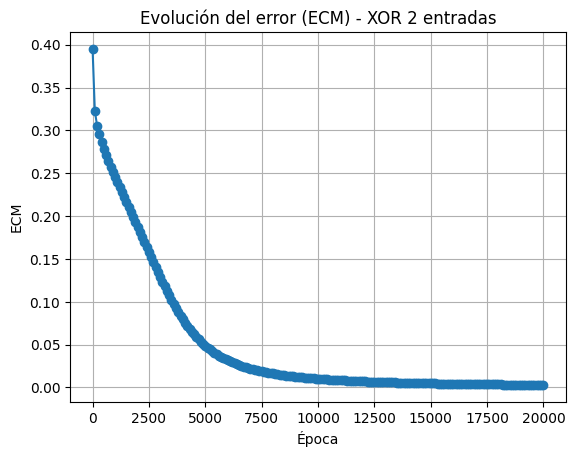
\includegraphics[width=0.7\linewidth]{../imgs/ej3/10neur/2ecm}
	\caption{Error por época - XOR de 2 entradas - MLP 10 neuronas en capa oculta}
	\label{fig:2ecm}
\end{figure}

\begin{figure}[htbp!]
	\centering
	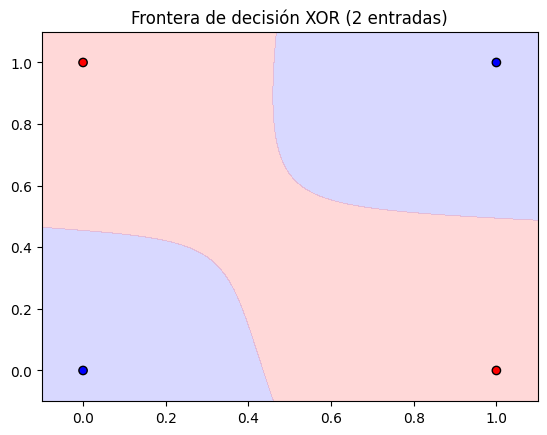
\includegraphics[width=0.7\linewidth]{../imgs/ej3/10neur/front}
	\caption{Frontera de decisión - XOR de 2 entradas - MLP 10 neuronas en capa oculta}
	\label{fig:front}
\end{figure}

\begin{figure}[htbp!]
	\centering
	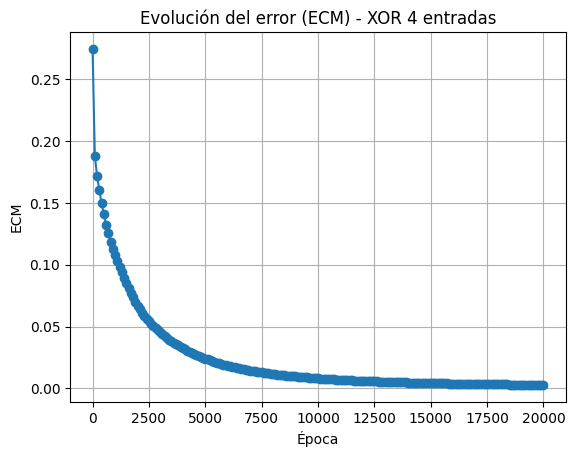
\includegraphics[width=0.7\linewidth]{../imgs/ej3/10neur/4ecm}
	\caption{Error por época - XOR de 4 entradas - MLP 10 neuronas en capa oculta}
	\label{fig:4ecm}
\end{figure}





\begin{table}[h!]
	\centering
	\begin{tabular}{cccc}
		\hline
		\textbf{Entradas} & \textbf{Target} & \textbf{Salida sigmoide} & \textbf{Predicción (umbral 0.5)} \\
		\hline
		$[0\ 0]$ & 0 & 0.051 & 0 \\
		$[0\ 1]$ & 1 & 0.948 & 1 \\
		$[1\ 0]$ & 1 & 0.942 & 1 \\
		$[1\ 1]$ & 0 & 0.057 & 0 \\
		\hline
	\end{tabular}
	\caption{Resultados del perceptrón con dos entradas y 10 neuronas ocultas.}
\end{table}

\begin{table}[h!]
	\centering
	\begin{tabular}{cccc}
		\hline
		\textbf{Entradas} & \textbf{Target} & \textbf{Salida sigmoide} & \textbf{Predicción (umbral 0.5)} \\
		\hline
		$[-1\ -1\ -1\ -1]$ & 0 & 0.113 & 0 \\
		$[1\ -1\ -1\ -1]$ & 1 & 0.950 & 1 \\
		$[-1\ 1\ -1\ -1]$ & 1 & 0.931 & 1 \\
		$[1\ 1\ -1\ -1]$ & 0 & 0.028 & 0 \\
		$[-1\ -1\ 1\ -1]$ & 1 & 0.912 & 1 \\
		$[1\ -1\ 1\ -1]$ & 0 & 0.018 & 0 \\
		$[-1\ 1\ 1\ -1]$ & 0 & 0.062 & 0 \\
		$[1\ 1\ 1\ -1]$ & 0 & 0.003 & 0 \\
		$[-1\ -1\ -1\ 1]$ & 1 & 0.921 & 1 \\
		$[1\ -1\ -1\ 1]$ & 0 & 0.042 & 0 \\
		$[-1\ 1\ -1\ 1]$ & 0 & 0.017 & 0 \\
		$[1\ 1\ -1\ 1]$ & 0 & 0.017 & 0 \\
		$[-1\ -1\ 1\ 1]$ & 0 & 0.012 & 0 \\
		$[1\ -1\ 1\ 1]$ & 0 & 0.010 & 0 \\
		$[-1\ 1\ 1\ 1]$ & 0 & 0.006 & 0 \\
		$[1\ 1\ 1\ 1]$ & 0 & 0.052 & 0 \\
		\hline
	\end{tabular}
	\caption{Resultados del perceptrón con cuatro entradas y 10 neuronas ocultas.}
\end{table}

\clearpage

\subsection{Análisis}

El análisis ya se desarrolló casi completamente en cada subsección. Lo que se puede afirmar es que la función XOR de 2 entradas es relativamente simple de aprender para un MLP (3 perceptrones mínimo, 2 en la capa oculta), pero no tanto la XOR de 4 entradas, que requirió de una capa oculta bastante más grande. Esto demuestra que siguen existiendo limitaciones a la cantidad de patrones que puede aprender una cierta red de perceptrones, y que parecería aumentar con la cantidad de neuronas agregadas.

Algo que no se mencionó es que los errores tienen forma de exponenciales decrecientes (aunque a veces deformes), que es normal para estos casos. Algunos entrenamientos presentaron como puntos silla, lo que indicaría que el algoritmo se encontró con una región de gradiente muy pequeño, como la figura \ref{fig:xor2err}, que se quedó varias epochs en 0.25 de ECM.



\section{Ejercicio 4}

\subsection{Consignas}

a - Implemente una red con aprendizaje Backpropagation que aprenda la siguiente función:
$$
f (x , y , z)= \sin(x)+\cos(y)+z
$$

Donde: $x$ e $y$ $\in [0,2 \pi]$ y $z \in [-1,1]$.

Para ello construya un conjunto de datos de entrenamiento y un conjunto de evaluación. Muestre la evolución del error de entrenamiento y de evaluación en función de las épocas de entrenamiento.

b - Estudie la evolución de los errores durante el entrenamiento de una red con una capa oculta de 30 neuronas cuando el conjunto de entrenamiento contiene 40 muestras. ¿Que ocurre si el minibatch tiene tamaño 40? ¿Y si tiene tamaño 1?

\subsection{Desarrollo}

El conjunto de datos se generó sin mayores problemas, fue solo evaluar la función $f(x,y,z)$ en muchos puntos.

Los datasets de entrnamiento y testeo se separaron 70/30 (56000 muestras de entrenamiento) y se entrenó variando el tamaño de minibatch.


\subsection{Análisis}




\clearpage

\section{Ejercicio 5}

\subsection{Consignas}

Siguiendo el trabajo de Hinton y Salakhutdinov (2006), entrene una máquina restringida de Boltzmann con imágenes de la base de datos MNIST. Muestre el error de reconstrucción durante el entrenamiento, y ejemplos de cada uno de los dígitos reconstruidos.
\subsection{Desarrollo}

\subsection{Análisis}

\clearpage

\section{Ejercicio 6}

\subsection{Consignas}

Entrene una red convolucional para clasificar las imágenes de la base de datos MNIST.
¿Cuál es la red convolucional más pequeña que puede conseguir con una exactitud de al menos 90\% en el conjunto de evaluación? ¿Cuál es el perceptrón multicapa más pequeño que puede conseguir con la misma exactitud?

\subsection{Desarrollo}

\subsection{Análisis}


\clearpage

\section{Ejercicio 7}

\subsection{Consignas}

Entrene un autoencoder para obtener una representación de baja dimensionalidad de las imágenes de MNIST. Use dichas representaciones para entrenar un perceptrón multicapa como clasificador. ¿Cuál es el tiempo de entrenamiento y la exactitud del clasificador obtenido cuando parte de la representación del autoencoder, en comparación con lo obtenido usando las imágenes originales?

\subsection{Desarrollo}



entrenamiento final:
Epoch 1/30 | Loss=0.6624 | Acc=81.28%
Epoch 2/30 | Loss=0.3537 | Acc=89.86%
Epoch 3/30 | Loss=0.3200 | Acc=90.68%
Epoch 4/30 | Loss=0.3073 | Acc=90.92%
Epoch 5/30 | Loss=0.2996 | Acc=91.19%
Epoch 6/30 | Loss=0.2962 | Acc=91.22%
Epoch 7/30 | Loss=0.2921 | Acc=91.29%
Epoch 8/30 | Loss=0.2884 | Acc=91.44%
Epoch 9/30 | Loss=0.2884 | Acc=91.51%
Epoch 10/30 | Loss=0.2855 | Acc=91.53%
Epoch 11/30 | Loss=0.2832 | Acc=91.62%
Epoch 12/30 | Loss=0.2837 | Acc=91.56%
Epoch 13/30 | Loss=0.2823 | Acc=91.63%
Epoch 14/30 | Loss=0.2813 | Acc=91.79%
Epoch 15/30 | Loss=0.2810 | Acc=91.69%
Epoch 16/30 | Loss=0.2799 | Acc=91.83%
Epoch 17/30 | Loss=0.2785 | Acc=91.79%
Epoch 18/30 | Loss=0.2773 | Acc=91.82%
Epoch 19/30 | Loss=0.2772 | Acc=91.85%
Epoch 20/30 | Loss=0.2775 | Acc=91.76%
Epoch 21/30 | Loss=0.2751 | Acc=91.91%
Epoch 22/30 | Loss=0.2738 | Acc=91.90%
Epoch 23/30 | Loss=0.2745 | Acc=91.89%
Epoch 24/30 | Loss=0.2738 | Acc=91.94%
Epoch 25/30 | Loss=0.2735 | Acc=91.97%
...
Epoch 28/30 | Loss=0.2736 | Acc=91.98%
Epoch 29/30 | Loss=0.2726 | Acc=91.98%
Epoch 30/30 | Loss=0.2720 | Acc=92.05%
Test Accuracy: 92.33%




\subsection{Análisis}

\clearpage


\section{Conclusiones}

\end{document}
